\chapter{Computation of subgraph similarity}

	In this chapter we present four different theoretical algorithm to compute subgraphs similarity as previously defined: an exhaustive enumeration, two similar randomized approach using the tools described in the previous chapter and a naive randomized approach.\\
	
	In the following algorithms, we will make use of parallel instruction, but we leave the specific programming choices and the comparison among the different approaches in the next chapter.
	
% \section{Calculation of indices}
%%%%%%%%%%%%%%%%%%%%%%%%%%%%%%%%%%%%%%%%%%%%%%%%%%%%%%%%%%%%%%%%%%%%%%%%%%%%%%%%%%%%%%%%%%%%%%%%%%%%%%%%%%%%%%%%%%%%
%%%%%%%%%%%%%%%%%%%%%%%%%%%%%%%%%%%%%%%%%%%%%%%%%%%%%%%%%%%%%%%%%%%%%%%%%%%%%%%%%%%%%%%%%%%%%%%%%%%%%%%%%%%%%%%%%%%%
\section{Indices calculation}

Now we illustrate the procedures to calculate the Frequency Jaccard and Bray-Curtis indices, as they are independent from the next algorithms we will present.\\

As previously seen, instead of iterate over all the strings in $\Sigma^{q}$ we can restrict to $\mathcal{L} \subseteq \Sigma^{q}$, the set of all possible $q$-grams found in the $q$-paths of $G$. 

An additional improvement can be made: if we want to calculate the similarity between two set $A, B \subset V$ ranging over $\mathcal{W} = \{ x \in \Sigma^{q} : x \in L(A) \text{ or } x \in L(B) \} \subseteq \Sigma^{q}$ it is enough, as we can easily see that for $x \in ( \Sigma^{q} \setminus \mathcal{W} )$ both $f_A[x]$ and $f_B[x]$ are equal to zero.\\

A last note, we can observe that in the Frequency Jaccard index we don't have to explicitly calculate $f_{A \cup B}[x]$ and its summary, as the exact value of $R = \Sigma_{x \in \mathcal{W}} f_{A \cup B}[x]$ can be easily calculate from $f_{A}[x] \text{ and } f_{B}[x]$.\\

So we define the following procedures:\\

\begin{algorithm}[h]
	\small
	\DontPrintSemicolon
	\SetKwInOut{Input}{Input}
	\SetKwInOut{Output}{Output}
	\Input{$\mathcal{W} = $ dictionary of $q$-grams\\$f_{A}[x] = $ frequency of each $x \in \mathcal{W}$ in $A$\\$f_{B}[x] = $ frequency of each $x \in \mathcal{W}$ in $B$}
	\Output{$BC(A,B) = $ the similarity between $A$ and $B$ according to Bray-Curtis index}
	\BlankLine
	$num \gets 0$\;
	$den \gets 0$\;
	\ForEach{$x \in \mathcal{W}$}{
		$num \gets num + 2 \times \min( f_{A}[x], f_{B}[x] )$\;
		$dem \gets den + f_{A}[x] + f_{B}[x]$\;
	}
	$BC \gets \frac{num}{den}$\;
	\Return{$BC$}
	\caption{\textsc{Bray-Curtis}}
	\label{alg:bray-curtis}
\end{algorithm}


\begin{algorithm}[h]
	\small
	\DontPrintSemicolon
	\SetKwInOut{Input}{Input}
	\SetKwInOut{Output}{Output}
	\Input{$\mathcal{W} = $ dictionary of $q$-grams\\$f_{A}[x] = $ frequency of each $x \in \mathcal{W}$ in $A$\\ $f_{B}[x] = $ frequency of each $x \in \mathcal{W}$ in $B$\\ $R =$ summation of all frequency}
	\Output{$FJ(A,B) = $ the similarity between $A$ and $B$ according to Frequency Jaccard index}
	\BlankLine
	$num \gets 0$\;
	\ForEach{$x \in \mathcal{W}$}{
		$num \gets num + \min( f_{A}[x], f_{B}[x] )$\;
	}
	$FJ \gets \frac{num}{R}$\;
	\Return{$FJ$}
	\caption{\textsc{Frequency-Jaccard}}
	\label{alg:jaccard}
\end{algorithm}

In the next algorithms we focus only to compute the values of $\mathcal{W}$, $f_{A}[x]$, $f_{B}[x]$ and $R$.

\clearpage 
%%%%%%%%%%%%%%%%%%%%%%%%%%%%%%%%%%%%%%%%%%%%%%%%%%%%%%%%%%%%%%%%%%%%%%%%%%%%%%%%%%%%%%%%%%%%%%%%%%%%%%%%%%%%%%%%%%%%
%%%%%%%%%%%%%%%%%%%%%%%%%%%%%%%%%%%%%%%%%%%%%%%%%%%%%%%%%%%%%%%%%%%%%%%%%%%%%%%%%%%%%%%%%%%%%%%%%%%%%%%%%%%%%%%%%%%%
\section{Naive approach}

	The naive approach consists in enumerate all the possible $q$-grams of simple $q$-paths leading to $u \in A \cup B$. 
	This can be done by starting a modified $\textsc{dfs}$ for each $u \in A \cup B$.
	
    \begin{algorithm}[h]
    \small
    \DontPrintSemicolon
    \SetKwInOut{Input}{Input}
    \SetKwInOut{Output}{Output}
    \Input{$q = $ length of the paths\\$A, B = $ set of nodes to compare}
	\Output{$\mathcal{W} = $ dictionary of $q$-grams\\$f_{A}[x] = $ frequency of each $x \in \mathcal{W}$ in $A$\\ $f_{B}[x] = $ frequency of each $x \in \mathcal{W}$ in $B$\\ $R =$ summation of all frequency}
    \BlankLine
    $R \gets 0$\;
	$\mathcal{W} \gets \emptyset$\;
	$f_{A \cup B} \gets \emptyset$ \quad \;    
	$f_{A} \gets \emptyset$\; 
	$f_{B} \gets \emptyset$\; 
	\BlankLine
    \textbf{parallel} \ForEach{$u \in A \cup B$}{
		$\langle \mathcal{W}_{u}, f_{u} \rangle \gets \textsc{DFS}(\langle u \rangle, q)$\;
		$\mathcal{W} \gets \mathcal{W} \cup \mathcal{W}_{u}$\;
		$f_{A \cup B} \gets f_{A \cup B} \cup f_{u}$\;
	}
	\BlankLine    
	\ForEach{$\langle u, x \rangle \in f_{A \cup B}$}{ 
		$R \gets R + f_{A \cup B}[\langle u, x \rangle]$\;
		\If{$u \in A$}{
			$f_{A}[x] \gets f_{A}[x] + f_{A \cup B}[\langle u, x \rangle]$\;
		}
		\If{$u \in B$}{
			$f_{B}[x] \gets f_{B}[x] + f_{A \cup B}[\langle u, x \rangle]$\;
		}
	}
	\BlankLine
    \Return{$\langle \mathcal{W}$, $f_{A}[x]$, $f_{B}[x]$, $R \rangle$}
    \caption{\textsc{brute-force}}
    \label{alg:brute-force}
    \end{algorithm}

	Note that, as we have to separate the frequencies between $f_{A}$ and $f_{B}$, the type of $f_{A \cup B}$ is not a map $ \Sigma^{q} \rightarrow \mathbb{N}$
	but instead is a map $V \times \Sigma^{q} \rightarrow \mathbb{N}$, where the element in $V$ is the leading node of the $q$-path associated to the $q$-gram.\\ 
	
	The values of $FJ(A,B)$ and $BC(A,B)$ calculated using this method are exact, we will use it only to compare the precision of the following approaches as it found all the possibile $O(|\Sigma|^{q})$ $q$-gram with a complexity of $O(|V|^{q})$.\\
	
	\clearpage
	
	For completeness we also illustrate the modified $\textsc{DFS}$ algorithm that keeps track of the current $q$-path and the relative $q$-gram.
	
    \begin{algorithm}[h]
		\small
		\DontPrintSemicolon
		\SetKwInOut{Input}{Input}
		\SetKwInOut{Output}{Output}
		\Input{$\pi = \langle u_{1}, \ldots, u_{|\pi|} \rangle $ current traversing path of length $\leq q$ \\$q = $ length of the paths }
		\Output{$\mathcal{W} =$ dictionary of $q$-grams of $q$-path having $\pi$ as suffix\\$f_{u}[x] = $ frequency of each $x \in \mathcal{W}$  }
		\BlankLine
		$\mathcal{W} \gets \emptyset$\;
		$f_{u} \gets \emptyset$ \quad \;    
		\BlankLine
		\If{$|\pi| = q$}{
			$\mathcal{W} \gets \mathcal{W} \cup \{ L(\pi) \}$\;
			$f_{u}[\langle u_{q}, L(\pi) \rangle] \gets 1$\;
		}
		\Else{
			\ForEach{$v \in N(u_{1}) \setminus \pi$}{
				$\langle \mathcal{W}_{v}, f_{v} \rangle \gets \textsc{DFS}(\langle v \rangle \cdot \pi, q)$\;
				$\mathcal{W} \gets \mathcal{W} \cup \mathcal{W}_{v}$\;
				$f_{u} \gets f_{u} \cup f_{v}$\;
			}	
		}
		\BlankLine
		\Return{$\langle \mathcal{W}$, $f_{u} \rangle$}
		\caption{\textsc{DFS}}
		\label{alg:brute-force}
	\end{algorithm}

	Where the symbol $\cdot$ is the concatenation of paths, note that we put the node $v$ before the path $\pi$ as we are interested to find all the $q$-path leading to the original calling node $u$.
	
	As last thing, with $N(u_{1}) \setminus \pi$ we avoid to revisit the nodes already present in the path $\pi$, so we restrict to the simple $q$-paths.\\
	
	\begin{minipage}{0.6\textwidth}\raggedright
		\begin{esempio}
		\end{esempio}
		The call to the method $\textsc{DFS}(0, 3)$ return:\\
		
		$\mathcal{W} = \{ abc, acb, acc \}$\\
		$f_{u}[\langle 0, abc \rangle] = 4$ ($\textsc{0-1-3}$ $\textsc{0-1-4}$ $\textsc{0-2-3}$ $\textsc{0-2-4}$)\\
		$f_{u}[\langle 0, acb \rangle] = 2$ ($\textsc{0-4-1}$ $\textsc{0-4-2}$)\\
		$f_{u}[\langle 0, acc \rangle] = 1$ ($\textsc{0-4-3}$)\\
	\end{minipage}
	\begin{minipage}{0.35\textwidth}
		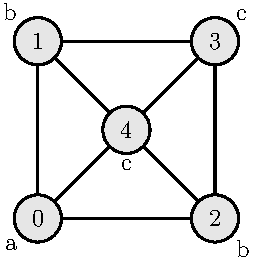
\includegraphics[width=\linewidth]{figure/figure-3-2}
	\end{minipage}
			
\clearpage

%%%%%%%%%%%%%%%%%%%%%%%%%%%%%%%%%%%%%%%%%%%%%%%%%%%%%%%%%%%%%%%%%%%%%%%%%%%%%%%%%%%%%%%%%%%%%%%%%%%%%%%%%%%%%%%%%%%%
%%%%%%%%%%%%%%%%%%%%%%%%%%%%%%%%%%%%%%%%%%%%%%%%%%%%%%%%%%%%%%%%%%%%%%%%%%%%%%%%%%%%%%%%%%%%%%%%%%%%%%%%%%%%%%%%%%%%
\section{Efficient computation}

% \clearpage

%%%%%%%%%%%%%%%%%%%%%%%%%%%%%%%%%%%%%%%%%%%%%%%%%%%%%%%%%%%%%%%%%%%%%%%%%%%%%%%%%%%%%%%%%%%%%%%%%%%%%%%%%%%%%%%%%%%%
%%%%%%%%%%%%%%%%%%%%%%%%%%%%%%%%%%%%%%%%%%%%%%%%%%%%%%%%%%%%%%%%%%%%%%%%%%%%%%%%%%%%%%%%%%%%%%%%%%%%%%%%%%%%%%%%%%%%
\subsection*{Color coding}

\begin{algorithm}[h]
	
	\small
	\DontPrintSemicolon
	\SetKwInOut{Input}{Input}
	\SetKwInOut{Output}{Output}
	\Input{\ $G = (V,E)$ undirected graph with $q$ random colors.}
	\Output{\ $M = $ dynamic programming table for color coding.}
	
	% $M\in [q]\times V$ is the dynamic programming table of color coding, where $M[i][u]$ is the set of pairs $C,f$ with $C\subseteq [q]$, $|C|=i$, and $f\in \mathds{N}$ such that $f$ is the number of paths having color set $C$ ending in $u$\;
	
	\BlankLine
	
	\textbf{parallel} \lForEach{$u \in V$}{$M_{1,u} = \langle \chi(u), 1 \rangle$}
	
	\For{$i \in \{ 2, 3, \ldots, q\}$}{
		\textbf{parallel} \ForEach{$u \in V$}{
			\ForEach{$v \in N(u)$}{
				\ForEach{$\langle C, f \rangle \in M_{i-1,v}$ such that $\chi(u) \not \in C$}{
					$f' \gets M_{i,u}\left(C \cup \{\chi(u)\}\right)$\;
					$M_{i,u} \gets \langle C \cup \{\chi(u)\}, f' + f \rangle$\;
				}
			}
		}   
	}
	\Return{$M$}
	%\setcounter{AlgoLine}{0}
	
	\caption{preprocess: \textsc{color-coding}}
	\label{alg:color-coding}
\end{algorithm}

\clearpage
%%%%%%%%%%%%%%%%%%%%%%%%%%%%%%%%%%%%%%%%%%%%%%%%%%%%%%%%%%%%%%%%%%%%%%%%%%%%%%%%%%%%%%%%%%%%%%%%%%%%%%%%%%%%%%%%%%%%
%%%%%%%%%%%%%%%%%%%%%%%%%%%%%%%%%%%%%%%%%%%%%%%%%%%%%%%%%%%%%%%%%%%%%%%%%%%%%%%%%%%%%%%%%%%%%%%%%%%%%%%%%%%%%%%%%%%%
\subsection*{Colorful sampling}

\begin{algorithm}[h]
	
	\small
	\DontPrintSemicolon
	\SetKwInOut{Input}{Input}
	\SetKwInOut{Output}{Output}
	\Input{\ $X =$ array of nodes from graph $G$; $M =$ color coding table for $G$; $r =$ number of colorful paths to sample.}
	\Output{\ $W = $ random sample set of colorful grams $x \in L(X)$ with probability $p_X(x)$.}
	
	%Let $M\in [q]\times V$ be the dynamic programming matrix of color coding, where $M[i][u]$ is the set of pairs $C,f$ with $C\subseteq [q]$, $|C|=i$, and $f\in \mathds{N}$ such that $f$ is the number of paths having color set $C$ ending in $u$\;
	
	$R \gets \{\}$\;
	\textbf{parallel} \For{$j\in [r]$}{
		$u\gets$ randomly chosen $v \in X$ with probability~$p_v = \frac{M_{q,v}([q])}{\sum_{z\in X} M_{q,z}([q])}$\label{line:sample}\;
		$P\gets \textsc{random-path-to}(u)$\;
		\lIf{$P\not\in R$}{$R \gets R \cup \{ P \}$ \quad //critical section}
		\lElse{$j\gets j-1$ \quad //repeat the step}
	}
	\Return{$W = \{ L(P) : P \in R \}$}
	%\setcounter{AlgoLine}{0}
	
	\BlankLine
	
	\SetKwProg{myproc}{Function}{}{}
	\myproc{\textsc{random-path-to}(u)}{
		$P\gets \langle u \rangle$\;
		$D\gets [q] \setminus \{\chi(u)\}$\;
		
		\For{$i \in \{q-1,\ldots, 1\}$}{
			%Let $N$ be the neighbors $v$ of $u$ s.t. $M[i][v]$ contains the set of colors $D$\;
			$u\gets$ randomly chosen $v \in N(u)$ with probability~$p_{v} = \frac{M_{i,v}(D) }{ \sum_{z\in N(u)} M_{i,z}(D)}$\;
			$P\gets u \cdot P$\;
			$D\gets D\setminus \{\chi(u)\}$\;
		}
		\Return{P}   
	}
	
	
	\caption{query: \textsc{colorful-sampler}}
	\label{alg:randomsample}
	\label{alg:sample}
\end{algorithm}

\clearpage
%%%%%%%%%%%%%%%%%%%%%%%%%%%%%%%%%%%%%%%%%%%%%%%%%%%%%%%%%%%%%%%%%%%%%%%%%%%%%%%%%%%%%%%%%%%%%%%%%%%%%%%%%%%%%%%%%%%%
%%%%%%%%%%%%%%%%%%%%%%%%%%%%%%%%%%%%%%%%%%%%%%%%%%%%%%%%%%%%%%%%%%%%%%%%%%%%%%%%%%%%%%%%%%%%%%%%%%%%%%%%%%%%%%%%%%%%
\subsection*{Frequency count}

\begin{algorithm}[h]
	
	\small
	\DontPrintSemicolon
	\SetKwInOut{Input}{Input}
	\SetKwInOut{Output}{Output}
	\Input{\ $X =$ array of nodes from graph $G$; $W = $ sample of its colorful $q$-grams.}
	\Output{\ $f_X[x] = $ frequency of each $x \in W$.}
	
	%Let $M\in [q]\times V$ be the dynamic programming matrix of color coding, where $M[i][u]$ is the set of pairs $C,f$ with $C\subseteq [q]$, $|C|=i$, and $f\in \mathds{N}$ such that $f$ is the number of paths having color set $C$ ending in $u$\;
	
	\BlankLine
	$T\gets[\,]$ \quad // step~$i=1$\; 
	\textbf{parallel} \ForEach{$u \in X$ such that $L(u)$ appears at the end of a $q$-gram in $W$}{
		$T \gets T \cup [\langle u, L(u), \{\chi(u) \} \rangle]$\;
	}
	
	\For{$i \in \{ 2, 3, \ldots, q\}$}{
		$T' \gets [\,]$\;
		\textbf{parallel} \ForEach{$\langle z, x, C \rangle \in T$}{
			\ForEach{$v \in N(z)$ such that $\chi(v) \not \in C$}{
				\If{$L(v) \cdot x$ is a suffix of a $q$-gram in $W$}{
					$T' \gets T' \cup [\langle v, L(v) \cdot x, C \cup \{\chi(v)\} \rangle]$  \quad //critical s.\;
				}
			}
		}   
		$T \gets T'$\;
	}
	$f_X \gets (0,\ldots,0)$\;
	\lForEach{$\langle z, x, C \rangle \in T$}{
		$f_X[x] \gets f_X[x]+1$
	}
	
	\Return{$f_X$}
	%\setcounter{AlgoLine}{0}
	
	\caption{f-count, exactly counting frequencies of sampled $q$-grams}
	\label{alg:frequency}
\end{algorithm}

\clearpage
%%%%%%%%%%%%%%%%%%%%%%%%%%%%%%%%%%%%%%%%%%%%%%%%%%%%%%%%%%%%%%%%%%%%%%%%%%%%%%%%%%%%%%%%%%%%%%%%%%%%%%%%%%%%%%%%%%%%
%%%%%%%%%%%%%%%%%%%%%%%%%%%%%%%%%%%%%%%%%%%%%%%%%%%%%%%%%%%%%%%%%%%%%%%%%%%%%%%%%%%%%%%%%%%%%%%%%%%%%%%%%%%%%%%%%%%%
\subsection*{Frequency sampling}

TODO 
% \clearpage

\clearpage
%%%%%%%%%%%%%%%%%%%%%%%%%%%%%%%%%%%%%%%%%%%%%%%%%%%%%%%%%%%%%%%%%%%%%%%%%%%%%%%%%%%%%%%%%%%%%%%%%%%%%%%%%%%%%%%%%%%%
%%%%%%%%%%%%%%%%%%%%%%%%%%%%%%%%%%%%%%%%%%%%%%%%%%%%%%%%%%%%%%%%%%%%%%%%%%%%%%%%%%%%%%%%%%%%%%%%%%%%%%%%%%%%%%%%%%%%
\subsection*{Estimating similarity indices}

TODO 
%  \clearpage

\clearpage
%%%%%%%%%%%%%%%%%%%%%%%%%%%%%%%%%%%%%%%%%%%%%%%%%%%%%%%%%%%%%%%%%%%%%%%%%%%%%%%%%%%%%%%%%%%%%%%%%%%%%%%%%%%%%%%%%%%%
%%%%%%%%%%%%%%%%%%%%%%%%%%%%%%%%%%%%%%%%%%%%%%%%%%%%%%%%%%%%%%%%%%%%%%%%%%%%%%%%%%%%%%%%%%%%%%%%%%%%%%%%%%%%%%%%%%%%
\section{Baseline algorithm}

In order to validate the effectiveness of our approach, we compare the previously seen algorithms against a naive randomized approach .



the baseline algorithm BASELINE, 
that finds random paths in a simple way,

\begin{algorithm}[h]
	
	\small
	\DontPrintSemicolon
	\SetKwInOut{Input}{Input}
	\SetKwInOut{Output}{Output}
	\Input{\ $X =$ array of nodes from graph $G$; $ r =$ number of paths to sample.}
	\Output{\ $f_X[x] = $ frequency of each $x \in W$, where $W = $ naive random sample multiset of $q$-grams for $X$.}
	
	$R\gets\{\}$\;
	\textbf{parallel} \For{$j\in [r]$}{
		$u\gets$ randomly chosen $v \in X$ with uniform probability\;
		$P\gets \textsc{naive-random-path-to}(u)$\;
		\lIf{$P \neq \mathtt{null}$ and $P\not\in R$}{$R \gets R \cup \{ P \}$ \quad //critical section}
		\lElse{$j\gets j-1$ \quad //repeat the step}
	}
	$W \gets [ L(P) : P \in R ]$\;
	$f_X \gets (0,\ldots,0)$\;
	\lForEach{$x \in W$}{
		$f_X[x] \gets f_X[x]+1$
	}
	\Return{$f_X$}
	%\setcounter{AlgoLine}{0}
	
	\BlankLine
	
	\SetKwProg{myproc}{Function}{}{}
	\myproc{\textsc{naive-random-path-to}(u)}{
		$P\gets \langle u \rangle$\;
		\For{$i \in \{q-1,\ldots, 1\}$}{
			\lIf{$N(u) \setminus P = \emptyset$}{return $\mathtt{null}$}
			$u\gets$ randomly chosen $v \in N(u) \setminus P$ with uniform prob.\;
			$P\gets u \cdot P$\;
		}
		\Return{P}   
	}
	
	\caption{\textsc{base}\xspace, the baseline sampler}
	\label{alg:baseline}
\end{algorithm}

\clearpage
